\section{Validation Metrics}
We found our pipeline to be an effective tool to beautify images of urban spaces. We now want to understand what the algorithm is looking at when transforming images. One way to do so would be to look at the template images and infer color and texture patterns. However, this approach is not scalable, as it would involve a substantial manual effort, and would be subject to personal interpretation. 
 
%
One of the main contributions of this work is to develop metrics%, which can to a high degree of certainty, 
to explain what the network is learning %to be   
as discriminatory features of beauty, in a fully automatic way. %We summarize some metrics mentioned in the table \ref{tab:Design_metrics}, which are taken from 
%urban design literature. 
%To test the different hypotheses, we use the balanced sample of 1000 images which rank on the extreme fringes of the Trueskill scores distribution and then transform these images towards the opposite side of the distribution . So an ugly image, according to its Trueskill score, would be transformed into a beautiful images and vice versa. Once the transformation is done, we measure different computational metrics and compare
%them between these two transformed groups. The differences in these metrics give us a good understanding of what the deep learning model is learning about the concept if beauty in an urban setting. 
Table \ref{tab:Design_metrics} shows a list of 5 evaluation metrics%, which are 
taken from urban design literature\cite{ewing2013measuring,alexander1977pattern}. These represent interpretable, measurable urban elements whose presence drives the aesthetic value of an urban environment. %Apart from being interpretable, these metrics also have an important property which is measurability. 
We design computer-based features to map each of these theoretical metrics into a computational form. 
To measure the metrics, we select 500 ugly and 500 beautiful images from the test dataset based on their base TrueSkill scores. We then transform these images towards the opposite side of the beauty specturm using the FaceLift pipeline. 
%This allows to measure in a fully automatic way t
We compare the values of these features between the two changed samples (beauty -> ugly , ugly->beauty), thus inferring statistics regarding which types of urban elements are added/removed by the beautification pipeline.
%All of these metrics have an approximate way of measurement using one or more of the computer the state of art computer vision tools. 
In this Section, we present the computational methods used to map these 5 metrics, as well as the results that we get on the pre and post transform images. 


\begin{table*}[h]
	\centering
	
	\resizebox{\linewidth}{!}{%
		\begin{tabular}{|c|p{14cm}|}
			\hline
			\textbf{Metric} & \textbf{Description}\\
			\hline
			Walkability  & Walkable streets are rated high on an aesthetic scale \cite{ewing2013measuring}. Walkable streets increase the social capital of a place and appeal to the exploring nature of human psyche. This implies that the urban space needs to address the fundamental need of people to walk and explore. This also implies that a walkable street must also be perceived as safe.\\
			\hline
			Green Spaces & Presence of Greenery is always pleasing to the eye. The literature always links urban beauty  to curated and well maintained green spaces, where social interactions can happen \cite{alexander1977pattern}. %, to be elements that bring a place 
			%together. 
			This 'social' aspect of greenery implies that dense forests or unkempt greens are not always related to the sense of beauty in urban scenes. \\
			\hline		
			Landmarks & Loosing a bearing in the city is not a very pleasant experience. Hence presence of recognisable and  guiding landmarks influences the perception of an urban space \cite{ewing2013measuring}.\\
			\hline
			Privacy-Openness &  A sense of privacy and a complimentary sense of openness are both influential in our perception of a place\cite{ewing2013measuring}. These values also tend to be related in an inverse 'U' fashion with beauty. \\ 
			\hline
			Visual Complexity & Visual complexity is a measure of how diverse a urban scene is. It manifests in terms of various design materials, textures and objects. Generally, visual complexity has an inverse 
			'U' relation with aesthetic values. The beauty and aesthetics of a place increases until it starts dropping because of 'too much' complexity\cite{ewing2013measuring}. \\
			\hline
	\end{tabular}}
	\caption{Urban Design Metrics \textbf{ADD IMPLEMENTATION INTO COMPUTATIONAL APPROACH}}
	\label{tab:Design_metrics}
	%        \vspace{-5mm}
\end{table*}


\subsection{Computational Methods}
To validate the presence before/after transformation of the 5 urban elements in Table \ref{tab:Design_metrics} we use a set computer-vision based tools as well as traditional data analysis techniques.


\subsubsection{Measuring Walkability and presence of Landmarks}
To quanitfy elements of Walkability, Greenery, and Landmarks, we proceed as follows. % %We use the data that is transformed into beautiful and ugly scenes using the learned model, to analyze scene level characteristics.
We use PlacesNet \cite{zhou2014learning} to extract information regarding the scene type (e.g. beach, garden, etc.). PlaceNet's output is the SoftMax distribution over 205 scene labels. We retain for an image the top 5 labels with higher confidence scores.
We classify the 205 scene labels of PlacesNet into 4 categories, \textbf{L}andmarks , \textbf{A}rchitectural , \textbf{W}alkable , \textbf{N}atural. Each category is inspired from  urban design literature \cite{urbanDesign}.  Labels like \textit{Abbey , Plaza , Courtyard, Garden, Picnic Area, Park , etc} fall into the category of \textit{Walkable}, where as labels like \textit{Mansion, Castle, Dam , Airport, etc} fall in the category of \textit{Landmarks}. Labels like \textit{Residential neighborhood, Motel, hotel, restaurant, etc} fall in the category of \textit{Architectural} and labels like {fields, pasture , forest, ocean, beach etc } fall in the category \textit{Natural}. %All in all 
For an image, we then measure its Wakability according to how many of the top-5 labels fall in category W. Similarly, we quantify presence of Greenery and Landmarks according to the frequency of N and L labels.%These higher-level LAWN labels represent  broader urban design motifs that constitute a liveable city we can detect through PlaceNEt. 

\subsubsection{Measuring Openness and Green spaces}
To measure Openness, we resort to   Segnet \cite{badrinarayanan2015segnet}, a semantic segmentation algorithm, which is trained on dashcam images from a real driving dataset , to detect 12 different elements in the image namely road, sky , trees ,  buildings , poles , signage , pedestrians, vehicles ,bicycles , pavement, fences and road markings. At the risk of over-simplifying, we can approximate that the openness of a street scene with the portion of sky visible in the scene, green cover by the portion of greenery detected in an image etc. We therefore quantify openness as the number of pixels labelled as 'sky' by segnet, and green cover as the portion of pixels labelled as greenery by segnet. 
%We visualize the trends in the portions of green or sky pixels by adopting the binned plot methodology. 

\subsubsection{Measuring Visual Complexity}
Visual complexity is a measure used in urban design measurement \cite{ewing2013measuring} to understand the diversity of a particular place. Ideally the complexity has a more granular nature, right from the texture of the roads and walls, to the groomed gardens or lack thereof. Again with a risk of over-simplication, but to approximate a computational metric, we define complexity as the amount of disorder in terms of distribution of urban elements in the scene. As described before, we use SegNet \cite{badrinarayanan2015segnet} , to extract a 12 dimensional stochastic vector consisting of the proportion of pixels belonging to each element for a given image.
For a given image, we store these proportions into a stochastic vector $XH(X)$ on that vector:
\begin{equation}
H(X) = -\sum p(i)\log p(i)
\label{eq:entropy} 
\end{equation}
The $i$ in Eq \ref{eq:entropy} is the SegNet dimension for one of the 12 objects. The entropy value $H(X)$ would become a proxy for visual complexity of the urban scenes. What we want to understand is not the absolute nature, but the trend in the variation of this value across the beautification process. 


\subsection{Testing Hypothesis}
We now try to reason about different hypothesis inspired from the literature \cite{ewing2013measuring,urbanDesign,alexander1977pattern} using the computational approaches mentioned above. The main outcome of this excercise is either to confirm or refute whether we can explain how our model understands beauty using popular urban design concepts. Without the loss of generalization, we want to probe whether the elements that the pipeline deems beautiful or ugly, are grounded in literature. 

\subsubsection{Walkability and Green spaces}
As mentioned in table \ref{tab:Design_metrics} , Walk-ability of streets has high impact on the beauty and other aesthetic qualities of a place. We test this by quantifying the amount of greenery and walkable elements added by the beautification process.
%We use this taxonomy to compare prevalence (i.e. over expression) of these scenes in beautified images compared to uglified images
First, we transform 500 images from both sides of the beauty spectrum to either beautiful (if ugly) or ugly (if beautiful) urban scenes. %We then find the range across which a particular metric varies across the 1000 images. 

After detecting LAWN categories through PlacesNet labels,  we compute, for each image, the difference between the category frequency before and after transformation (e.g. how many 'Walkable' labels are added after beautification?). We then plot the aggregated difference-distributions for beautified and uglified image sets in Fig \ref{fig:taxonomyCount}.% Because the transformation is directly dependent on maximizing the classifier's certainty about an image being beautiful or ugly, this method directly gives us a  beautiful or ugly urban scene.
%This method provides insights regarding how transformations change the presence of scene types.
\par
\textit{[H1] Walkable streets is favoured in beautiful urban scenes}
\par
To test that \textit{H1} is valid, we first plot a prevalence count of different categories of labels for Beautified and Uglified images. %These labels are scene types extracted using the PlacesNet deep convolutional network \cite{zhou2014learning}. The labels are then classified into taxonomical classes of Landmarks, Architectural, Walkable and Natural classes.  
It can be seen from Fig \ref{fig:taxonomyCount}, that walkable scene types are highly favoured in the beautification process. Ugly images are transformed into Walkable spaces almost twice as frequently in beautification compared uglification.
\begin{figure}[h]
	\centering
	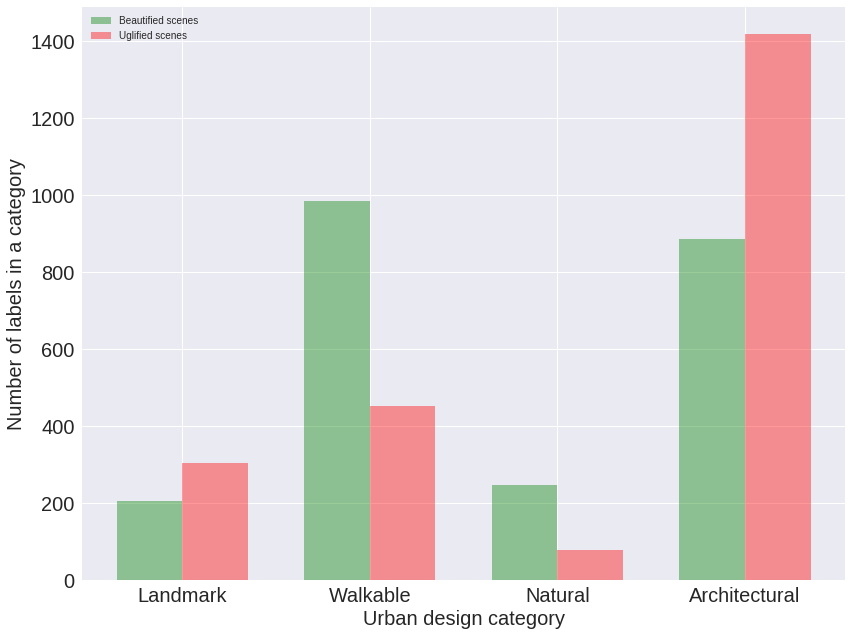
\includegraphics[width=\columnwidth]{Plot/taxonomyCount.png}
	\caption{Prevalence plot of categories of scenes prevalent in Beautified against Ugly-fied images}
	\label{fig:taxonomyCount}
\end{figure}

\par
\textit{[H2] Green spaces are favourable for beauty in urban scenes.  }
\par

Figure \ref{fig:taxonomyCount} and \ref{fig:WalkableTnomy} implies that natural scenes are twice as likely in beautified images than in uglified images. To test this hypothesis further, we further analyze the percentage of 'tree' pixels (according to SegNet) added by the beautification process: in average \textbf{[XXX\% pixels]} of greenery are added after beautification. %It can be seen from Fig \ref{fig:greenBinned} that more than as the green cover in an urban image increases, it is highly favoured in beautified class than in the u class. This shows that the green spaces are highly favourable for urban beauty.

\begin{figure}[h]
	\centering
	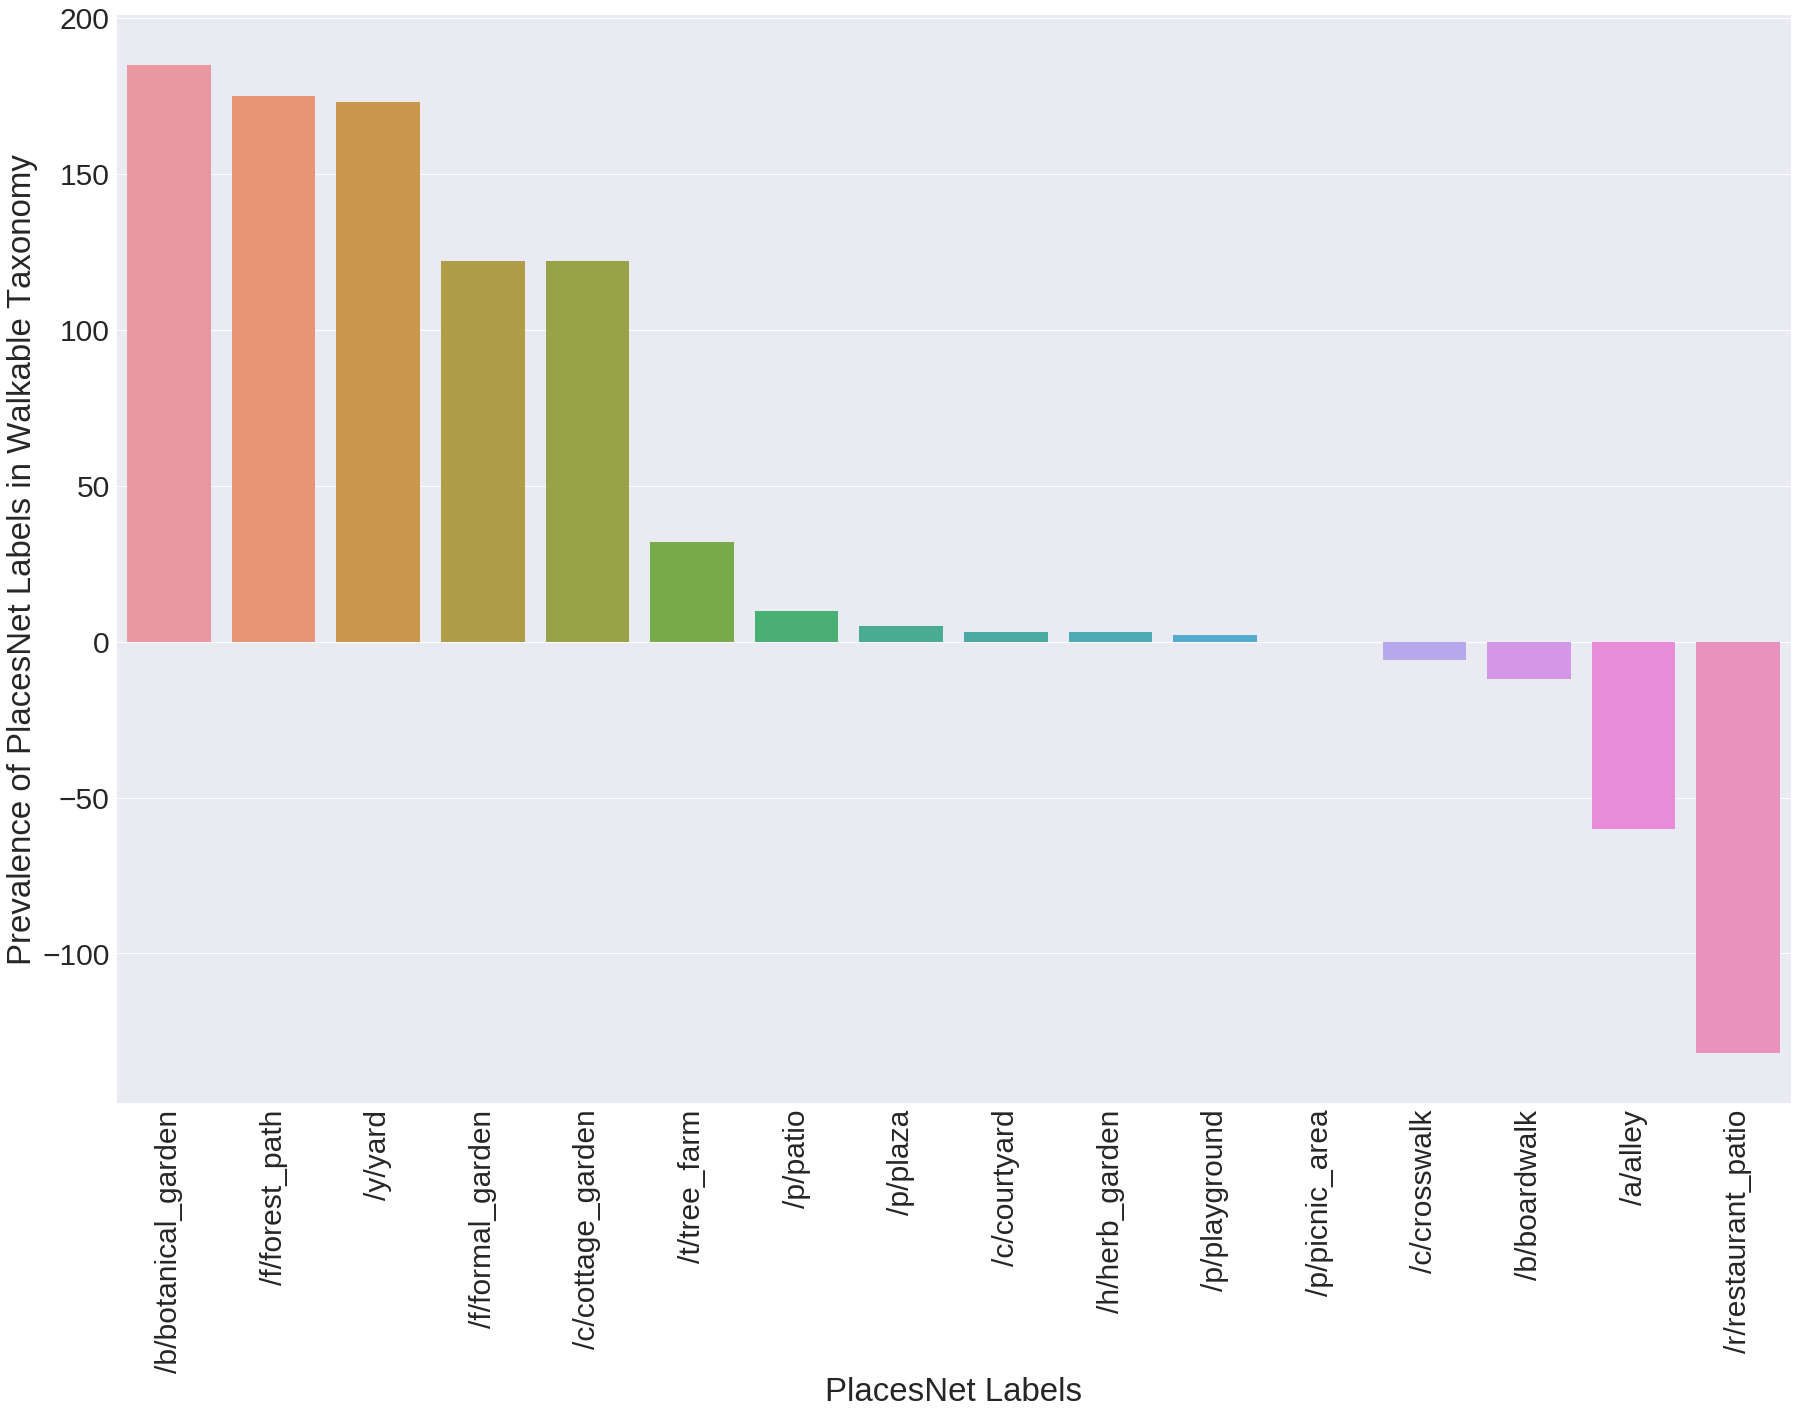
\includegraphics[width=\columnwidth]{Plot/walkable_taxonomy.png}
	\caption{Prevalence of Walkable labels in Beautified images against Ugly}
	\label{fig:WalkableTnomy}
\end{figure}

%\begin{figure}[h]
%	\centering
%	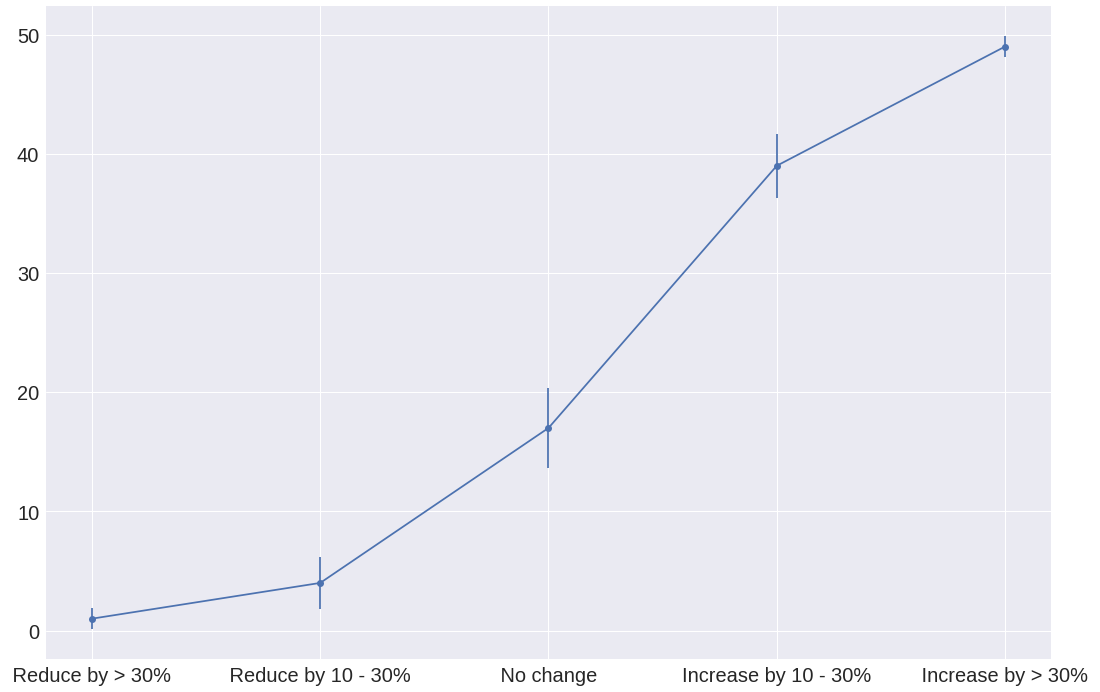
\includegraphics[width=\columnwidth]{Plot/Binned_deltas_trees.png}
%	\caption{Binned Plot for greenery pixels across transfomed images}
%	\label{fig:greenBinned}
%\end{figure}



\subsubsection{Privacy and  Openness }
\label{sec:privacy}

From the literature, it is conjectured that privacy is great when one
looks at personal spaces, but when it comes to public settings, there is an inverse 'U' relation with how private a place feels like. 
Too much privacy discourages the fundamental human urge to explore a mystery. Too much openness  alerts the primal urge to feel safe. 
\par
\textit{[H3] Sense of Privacy has an inverse 'U' relationship with the sense of beauty }
\par
What \textit{H3} suggests is that sense of privacy is not always associated with beauty. 
To understand the relationship between openness and beauty in urban scenes, we employ a technique called binned plots \textbf{CITE \cite{}}. We bin the range of sky pixels into \textbf{XXX Bins}%. This range is broken into bins and then each image out of the 1000, 
Each image is then assigned to the bin corresponding to its proportion of sky pixels. %, based on where the value of its metric falls. 
Among the 1000 images (500 uglified, 500 beautified) in our data, we then repeatedly sample 100 images across bins, and count how many of the sampled images fall in either beautified or uglified transformed category. We plot the mean and standard deviation in a plot for these occurrence frequencies. The resulting plot gives a trend about how likely is the presence of pixels favoured or disfavoured by the beautification process. 


\begin{figure*}[!t]
	\centering
	\hspace*{-5mm}
	\subfloat[]{
		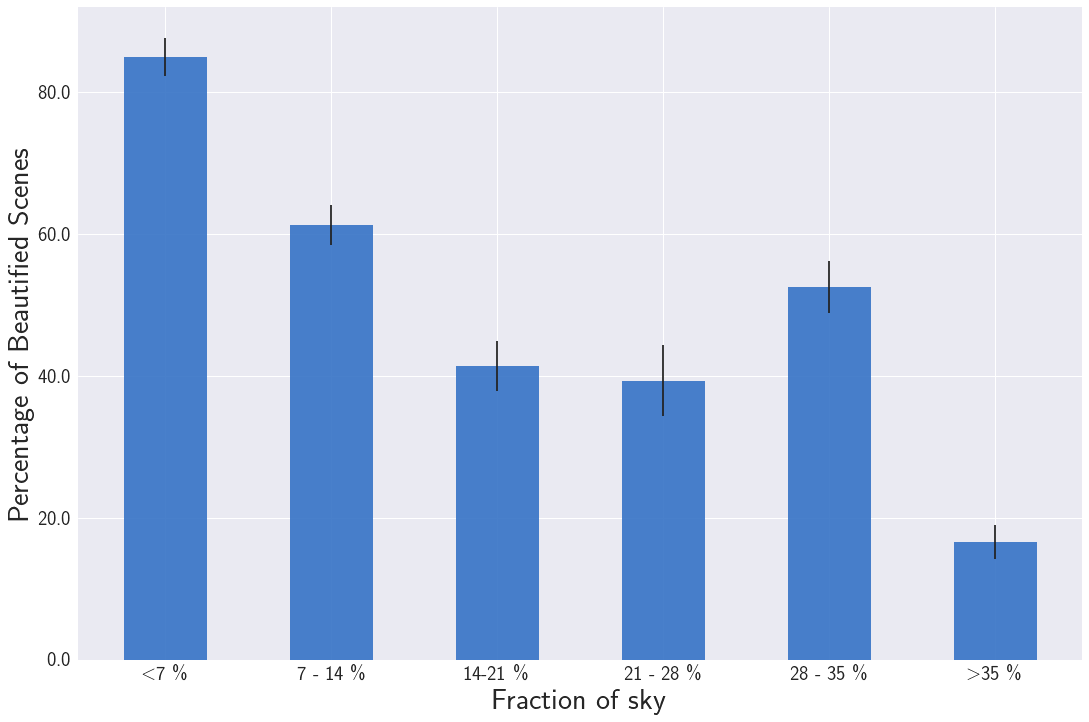
\includegraphics[width=0.45\textwidth, height = 5cm ]{Plot/BinnedPlot.png}
		\label{fig:greenBinned}
	}
	\subfloat[]{
		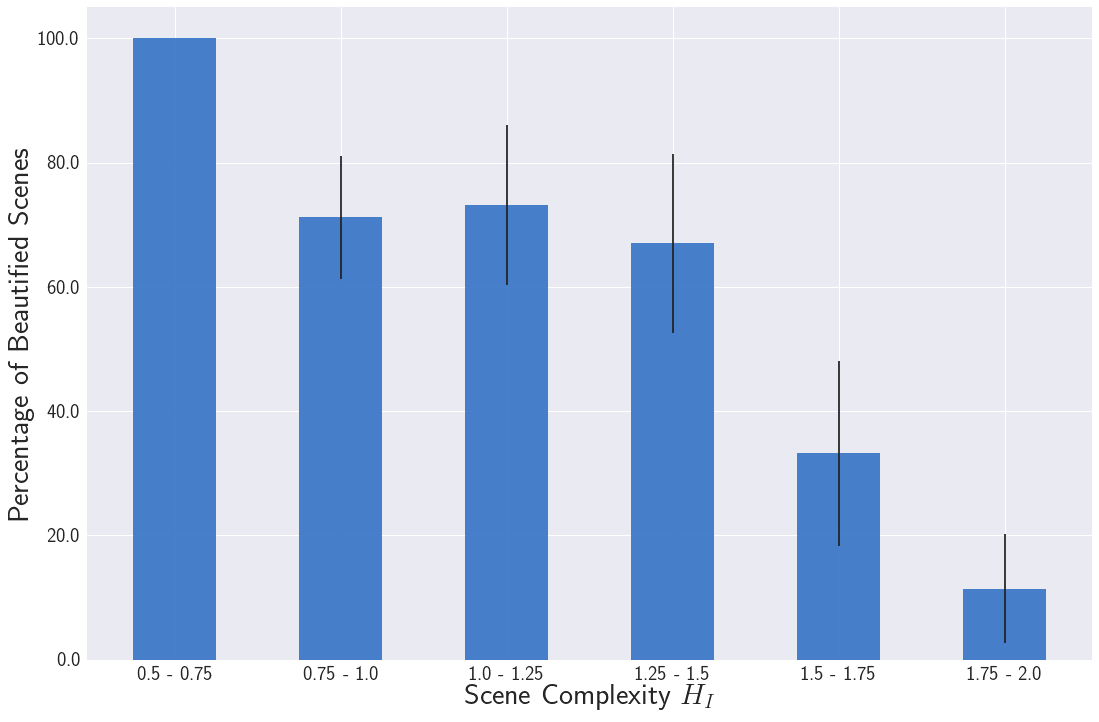
\includegraphics[width=0.45\linewidth, height = 5cm ]{Plot/binnedPlot_complexity.png}
		\label{fig:complexity}
	}
\vspace{-0.4cm}
\caption{ Figure \ref{fig:greenBinned} shows the Binned Plot for Sky pixels across transformed images and Figure \ref{fig:complexity} shows the Binned Plot for Visual Complexity across transformed images }
\vspace{-0.4cm}
\end{figure*}

%\begin{figure}[h]
%	\centering
%	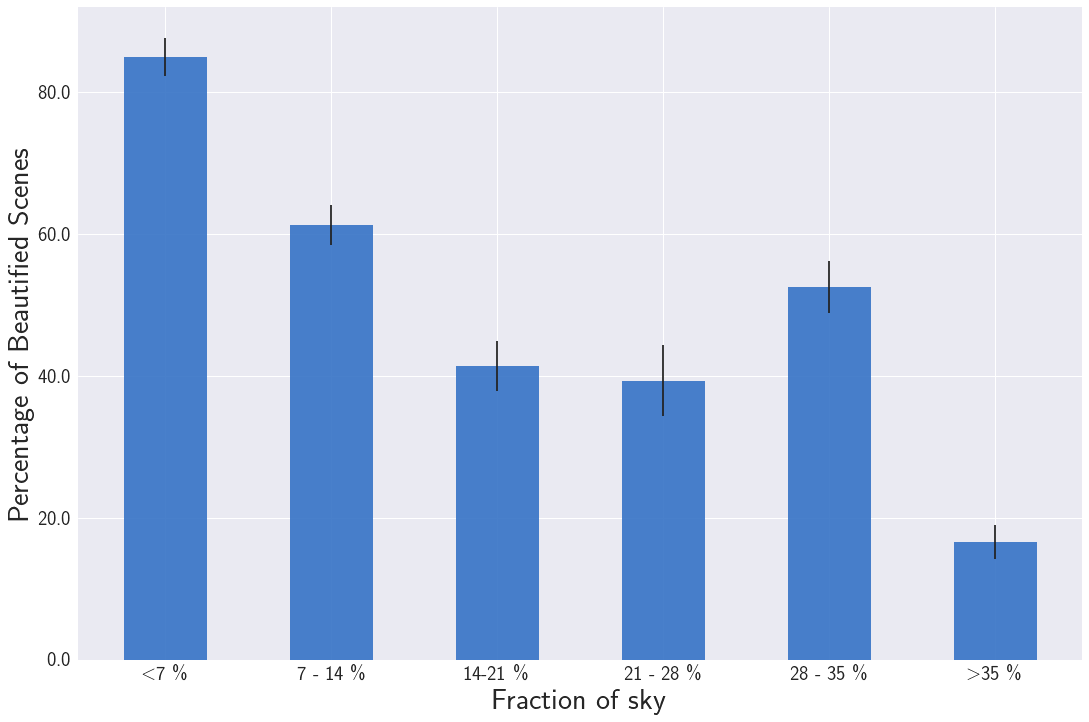
\includegraphics[width=\columnwidth]{Plot/BinnedPlot.png}
%	\caption{Binned Plot for Sky pixels across transformed images}
%	\label{fig:greenBinned}
%\end{figure}

It can be seen that our model prefers lack of openness in the beautification process. The inverse 'U' Relationship is completely absent and cozy urban places are actually favoured in the beautification process. 

%This effect can be individually seen from Fig \ref{fig:BuildingsCoverage} and Fig \ref{fig:TreeCoverage}. Beautification always prefers reduction of 
%visible buildings and increase in an overall green coverage \footnote{All distributions are tested using student-t tests and are found to have significantly hight T-statistic score (>>20) and p value << $10^{-5}$}. However this does not necessarily untangle the trade-off relationship of privacy-openness and beauty.

%To understand relation between openness and privacy, we repeat analysis as described in Section \ref{sec:vehicles}, for the amount of Sky and Tree pixels in a scene. The assumption here is these two objects in the scene are predominately driving the sense of openness. Adapting the Equation \ref{eq:regression} for the tree and sky pixel ratios we get different values for $\beta_1 , \beta_2 and \beta_3$. In this case the regression yields $\alpha = 0$ , $\beta_1 = 0.06$ , $\beta_2 = 0.10$ and $\beta_3 = -0.04$ . These values suggest that trees and sky, on their own have a positive impact on the beauty of a picture. 

\subsubsection{Visual Complexity }
Visual complexity is a metric to measure the diversity of an urban scene. There is a trade off  when it comes to balancing visual complexity with beauty. Too much diversity overwhelms the cognition and makes it hard to establish bearing. 
\par
\textit{[H4] Visual Complexity has a inverse 'U' relation with the sense of beauty }
\par

To test  this hypothesis, we compute the binned plot (see Sec. \label{sec:privacy}) of our complexity metric. It can be seen from Fig \ref{fig:complexity} that visual complexity does peak in beautiful images but then deteriorates rapidly.
%\begin{figure}[h]
%	\centering
%	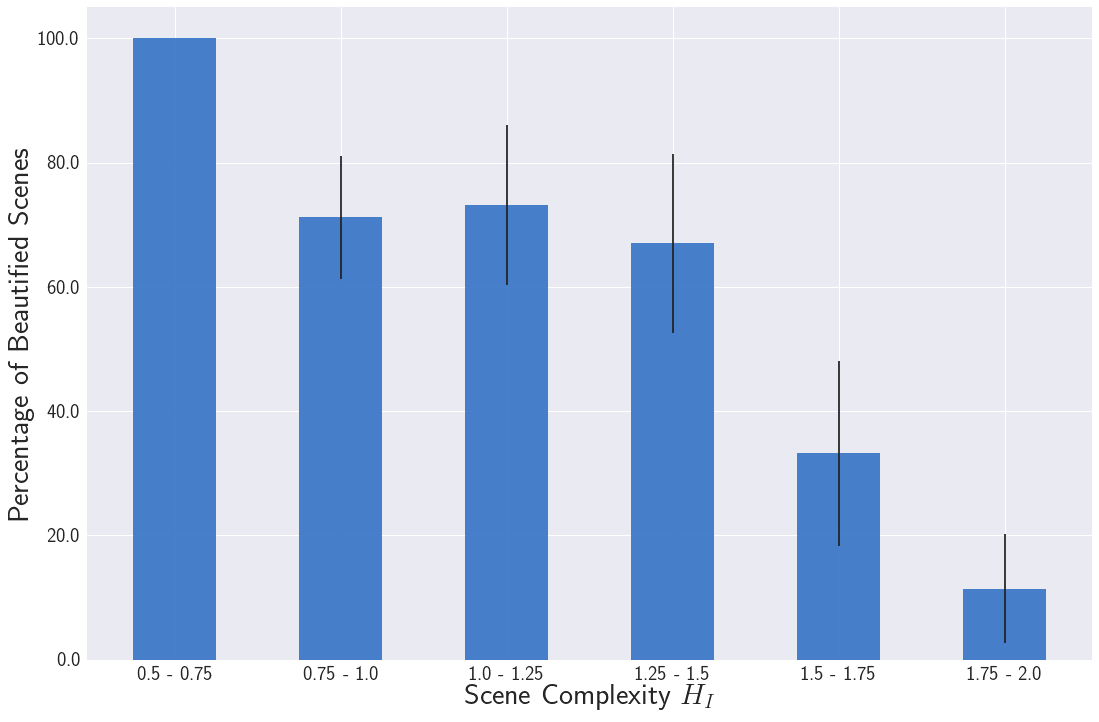
\includegraphics[width=\columnwidth]{Plot/binnedPlot_complexity.png}
%	\caption{Binned Plot for Visual Complexity across transformed images}
%	\label{fig:complexity}
%\end{figure}



\subsection{Interdependence of Urban elements}
To understand the predictability and interdependence between the most influencing objects in an image and the probability of finding an image beautiful, we adapt the approach as described in \cite{vaughn2008data},
which proposes using logistic regression coefficients as a measure for upper bounds on influence of a variable. This method is also helpful in understanding the interdependence of variables for a particular outcome. 
Using the approach we perform a logistic regression over the two variables $V_1$ and $V_2$ which denote the ratio of a particular type of object pixels to the total area of image in pixels. So these ratios basically represent how much of the total image area is dominated by a particular object. The objects in this study are limited to the 12 urban object labels supported by SegNet \cite{badrinarayanan2015segnet}.
Assuming dependence, we introduce  a third term, which represents the factor that measures the dependence of $V_1$ and $V_2$ and is simply the product $V_1 * V_2 $.
The logistic regression would try to fit a line 
\begin{equation}
L = invLogit(\alpha + \beta_1 * V_1 + \beta_2 * V_2  + \beta_3 * V_{1}.V_{2} )
\label{eq:regression} 
\end{equation}
Here $invLogit$ is the inverse Logistic function. According to the rule of fourth described in \cite{vaughn2008data} , the coefficients $ \beta_1, \beta_2 and \beta_3 $ represent some properties about the influence of $ V_1, V_2 $. An increase in 1\% area of the amount of pixels belonging to object $ V_2 $ would correspond to a maximum increase/decrease of $\frac{\beta_2}{4}$ percent in the likely hood of the image being beautiful. Same rule applies for $\beta_1$. In case of $\beta_3$ the co-efficient corresponds to mutual dependence. An intuitive explanation is that if a 1\% change in value of $V_1$ would add $\beta_3$ to the value of $\beta_2$. Hence $\beta_3$ links changes in variable $V_1$ to changes in influence of variable $V_2$ and vice versa.
We perform the logistic regression on the 5 prime influences namely \textit{Sky , Buildings , Road , Vehicles , Trees}. The results of pairwise regression along with the dependency term are summaries in the table \ref{tab:regressioncoef}
\begin{table}[h]
	\centering
	\begin{tabular}{|c|c|c|c|c|}
		\hline
		\textbf{Object pair} & \textbf{$\beta_1$}  & \textbf{$\beta_2$} & \textbf{$\beta_3$}  & Error Rate (Percentage)\\
		\hline
		\hline
		Roads - Vehicles  & -0.015  & -0.05 & 0.023  & 40.6 \\
		\hline
		Sky - Buildings & -0.08 & -0.11 & 0.064 & 14.4 \\
		\hline
		Sky - Trees & 0.03 & 0.11 & -0.012 & 12.8  \\
		\hline
		Buildings - Trees & -0.032 & 0.084  & 0.005  & 12.7 \\
		\hline
		Roads - Trees & 0.04  & 0.10 &  -0.031  & 13.5  \\
		\hline
		Roads - Buildings & -0.05  & -0.097  &  0.04  & 20.2  \\
		\hline
	\end{tabular}
	\caption{Regression coefficients}
	\label{tab:regressioncoef}
	%        \vspace{-5mm}
\end{table}


